\documentclass{beamer}
\usepackage{graphics}  % Add this in your document preamble
\usepackage[slovene]{babel}
\usetheme{Frankfurt}

\begin{document}

\title{Priprava predstavitve z okoljem Beamer}
\author[]{Robert Šeliga(23211220)}
\institute{Fakulteta za Strojništvo}
\titlegraphic{
\includegraphics[width=4 cm]{Slike/logo.png}}



\begin{frame}
  \titlepage
\end{frame}

\begin{frame}
  \frametitle{Kazalo}
  \tableofcontents
\end{frame}

\section{Uvod}
\begin{itemize}
    \item V tej predstavitvi boste izvedeli kako je potekala moja domača naloga pri predmetu Naparedna računalniška orodja.Naloga je zahtevala, da s pomočjo Monte Carlo izračunamo priblužek števila $\pi$
\end{itemize}

\section{Potek naloge}
\begin{frame}
  \frametitle{Potek naloge}
  \begin{itemize}
    \item s pomočjo metode Monte Carlo smo izračunali približno vrednost števila $\pi$.
\end{itemize}
\end{frame}

\subsection{Nadaljevaje poteka naloge}
\begin{frame}{Nadaljevaje poteka naloge}
    \begin{itemize}
    \item Metodo Monte Carlo smo reševali s pomočjo Metlaba, kot je prikazano na spodnji sliki
\end{itemize}
\begin{figure}
  \centering
  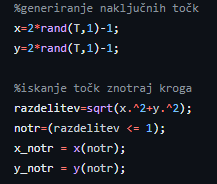
\includegraphics[width=0.5\textwidth]{Slike/MC1.png}
  \caption{Metoda Monte Carlo}
\end{figure}
\end{frame}

\subsection{Uporaba datotek in funkcij}
\begin{frame}{Uporaba datotek in funkcij}
    \begin{itemize}
    \item Morali smo uporabiti dve datoteki in eno funkcijo, ki so navedena spodaj:
    \begin{itemize}
        \item Funkcijska datoteka,
        \pause
        \item Programska datoteka,
        \pause
        \item Anonimna funkcija
    \end{itemize}
\end{itemize}
\end{frame}

\subsection{Izpis odstopanja in napake števila pi}
 \begin{frame}{Izpis odstopanja in napake pri $\pi$}
     \begin{itemize}
         \item Ob zagonu funkcije nam bo izpisalo kakšna je napaka in naš približek $\pi$, videli smo da je naša natančnost odvisna on našega števila točk. Večje kot bo število točk večja bo natančnost
         \begin{figure}
             \centering
             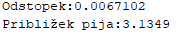
\includegraphics{Slike/izris.png}
             \caption{Izpis $\pi$(št. točk 4000)}
             \label{fig:Slika1}
         \end{figure}
     \end{itemize}
 \end{frame}

 \subsection{Izris točk}
 \begin{frame}{Izris točk}
 \begin{figure}
     \centering
     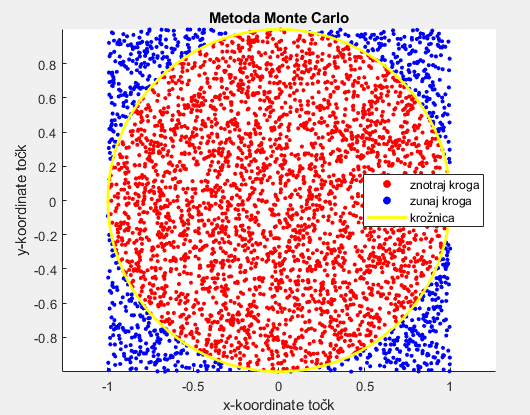
\includegraphics[width=0.9\textwidth]{Slike/tocke.png}
     \label{fig:Slika2}
 \end{figure}
     
 \end{frame}


\section{Zaključek}
\begin{frame}
  \frametitle{Zaključek}
  \begin{itemize}
    \item Ta domača naloga se mi zdi zelo zanimiva. Najboljše pa je, da sem se tako naučil novo metodo in dobil nekoliko boljšo predstavo glede števila $\pi$
  \end{itemize}
\end{frame}

\end{document}

